\documentclass[11pt, aspectratio=169, xcolor={dvipsnames}]{beamer}
\usepackage[utf8]{inputenc}
\usepackage[T1]{fontenc}
\usepackage{lmodern}
\usepackage{microtype}
\usepackage{graphicx}
\usepackage{tikz}
\usepackage{amsmath, amssymb, amsthm}
\usepackage{booktabs}
\usepackage{adjustbox}
\usepackage{ragged2e}

\usefonttheme{professionalfonts}

% Warm Professional Palette
\definecolor{DeepNavy}{HTML}{2E4057}
\definecolor{Teal}{HTML}{048A81}
\definecolor{WarmOrange}{HTML}{E85D04}
\definecolor{SoftPurple}{HTML}{9D4EDD}
\definecolor{WarmGray}{HTML}{6C757D}
\definecolor{LightGray}{HTML}{E9ECEF}
\definecolor{Cream}{HTML}{FBF8F1}
\definecolor{DeepRed}{HTML}{D62828}
\definecolor{Gold}{HTML}{D4A03A}
\definecolor{SoftWhite}{HTML}{FAFAFA}

% Beamer Theme Settings
\setbeamercolor{background canvas}{bg=Cream}
\setbeamercolor{normal text}{fg=DeepNavy}
\setbeamercolor{frametitle}{fg=DeepNavy, bg=Cream}
\setbeamercolor{title}{fg=DeepNavy}
\setbeamercolor{itemize item}{fg=Teal}
\setbeamercolor{itemize subitem}{fg=WarmOrange}

% No navigation symbols
\setbeamertemplate{navigation symbols}{}

% Frame title style: simple bold with lots of space
\setbeamertemplate{frametitle}{
    \vspace*{0.5cm}
    {\Large\bfseries\insertframetitle}
    \par
}

% Title page
\setbeamertemplate{title page}{
    \vfill
    {\huge\bfseries\inserttitle\par}
    \vspace{0.5cm}
    {\Large\insertauthor\par}
    \vspace{0.5cm}
    {\small\insertdate\par}
    \vfill
}

% Itemize style
\setbeamertemplate{itemize item}{\tikz\fill[Teal] (0,0) circle (0.12cm);}
\setbeamertemplate{itemize subitem}{\tikz\fill[WarmOrange] (0,0) circle (0.08cm);}

% Transition slide macro
\newcommand{\transitionslide}[2]{
    \begingroup
    \setbeamercolor{background canvas}{bg=DeepNavy}
    \setbeamercolor{normal text}{fg=Cream}
    \begin{frame}[c, plain]
        \centering
        {\Huge\bfseries\color{Cream} #1}
        
        \vspace{0.5cm}
        {\Large\color{Teal} #2}
    \end{frame}
    \endgroup
}

% TikZ Styles
\tikzset{
  cyclebox/.style={rectangle, draw=DeepNavy, thick, fill=SoftWhite,
                minimum width=3.5cm, minimum height=1cm,
                align=center, font=\small},
  cyclearrow/.style={->, thick, DeepNavy, #1},
}

\RaggedRight


\title{A Distributional Framework for Matched Employer Employee Data}
\author{Bonhomme, Lamadon, and Manresa (2019)}
\date{}

\begin{document}

\begin{frame}
    \titlepage
\end{frame}

\begin{frame}
    \frametitle{Estimating wage dispersion in short panels suffers from severe bias}
    
    In short panels (e.g., 2--4 years), the number of job movers per firm is often too small to reliably estimate individual firm fixed effects.
    
    \vspace{0.5cm}
    This leads to \textbf{incidental parameter bias}:
    \begin{itemize}
        \item Overstating the variance of firm effects
        \item Understating (or finding negative) correlation between worker and firm effects
        \item Masking true sorting patterns in the data
    \end{itemize}
\end{frame}

\begin{frame}
    \frametitle{We want to measure sorting, but standard tools force us to assume it away}
    
    Structural search and matching models (e.g., Shimer and Smith, 2000) emphasize:
    \begin{itemize}
        \item \textbf{Complementarities}: Different workers rank identical firms differently.
        \item \textbf{Endogenous mobility}: The decision to move depends on the current wage.
        \item \textbf{State dependence}: The previous firm impacts the wage at the next firm.
    \end{itemize}
    
    \vspace{0.5cm}
    But empirical tractability usually forces us to use two-way fixed effects models that assume away all of these mechanisms.
\end{frame}

\transitionslide{The Model and Intuition}{Bridging the gap}

\begin{frame}
    \frametitle{The AKM model relies on additive separability}
    
    The standard AKM (Abowd, Kramarz, and Margolis, 1999) specification:
    
    \[ Y_{it} = \alpha_i + \psi_{j(i,t)} + X_{it}'\beta + \varepsilon_{it} \]
    
    \vspace{0.5cm}
    \textbf{Strong Implications:}
    \begin{itemize}
        \item Log-earnings are strictly additive in worker and firm components.
        \item No complementarities in production or wage setting.
        \item Strict exogeneity: Mobility does not depend on wage realizations $\varepsilon_{it}$.
        \item No state dependence: Once you move to firm $j$, your previous firm $j'$ doesn't matter.
    \end{itemize}
\end{frame}

\begin{frame}
    \frametitle{Reducing firm heterogeneity to classes preserves parsimony}
    
    Instead of individual firm effects $\psi_j$, assume firms belong to $K$ unobserved \textbf{classes}.
    
    \vspace{0.5cm}
    Let $k_{it} = k(j_{it}) \in \{1, \dots, K\}$ be the class of the firm where worker $i$ works at time $t$.
    
    \vspace{0.5cm}
    By moving the dimensionality problem from $J$ (firms) to $K$ (classes), we can:
    \begin{itemize}
        \item Overcome the incidental parameter bias
        \item Allow for complex interactions between worker types and firm classes
        \item Model dynamic wage paths and mobility decisions
    \end{itemize}
\end{frame}

\begin{frame}
    \frametitle{The static model allows for non-additive interactions}
    
    Worker $i$ has an unobserved discrete type $\alpha_i \in \{1, \dots, L\}$.
    
    \vspace{0.5cm}
    A flexible interactive wage equation:
    \[ Y_{it} = a_t(k_{it}) + b_t(k_{it})\alpha_i + X_{it}'c_t + \varepsilon_{it} \]
    
    \vspace{0.5cm}
    If $b_t(k) = 1$ for all $k$, we recover the AKM model (at the class level). If $b_t(k)$ varies, the model captures complementarities.
\end{frame}

\begin{frame}
    \frametitle{The dynamic model introduces endogenous mobility and state dependence}
    
    In the dynamic extension:
    \begin{itemize}
        \item \textbf{Endogenous Mobility:} The probability of moving $m_{it}$ and the destination class $k_{it+1}$ depend on the \textit{current wage} $Y_{it}$, not just the firm class.
        \item \textbf{State Dependence:} The new wage $Y_{it+1}$ depends on the \textit{previous wage} $Y_{it}$ and the \textit{previous firm class} $k_{it}$.
    \end{itemize}
    
    \vspace{0.5cm}
    This is formulated as a first-order Markov process for wages, firm classes, and mobility.
\end{frame}

\begin{frame}
    \frametitle{Wage functions are identified by observing workers moving across classes}
    
    How do we identify complementarities? By looking at job movers.
    
    \vspace{0.5cm}
    \begin{center}
    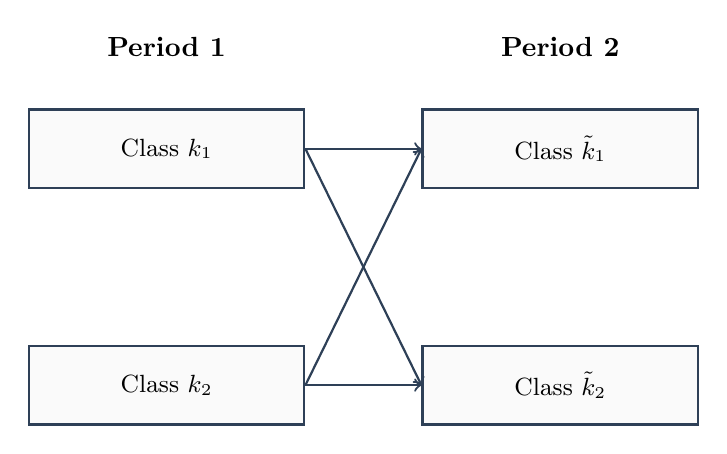
\begin{tikzpicture}
    % Coordinate map:
    % (K1T1) at (0, 1.5)  — 3.5cm x 1cm — "Class k_1"
    % (K2T1) at (0, -1.5) — 3.5cm x 1cm — "Class k_2"
    % (K1T2) at (5, 1.5)  — 3.5cm x 1cm — "Class \tilde{k}_1"
    % (K2T2) at (5, -1.5) — 3.5cm x 1cm — "Class \tilde{k}_2"
    
    \node[cyclebox] (K1T1) at (0, 1.5) {Class $k_1$};
    \node[cyclebox] (K2T1) at (0, -1.5) {Class $k_2$};
    \node[cyclebox] (K1T2) at (5, 1.5) {Class $\tilde{k}_1$};
    \node[cyclebox] (K2T2) at (5, -1.5) {Class $\tilde{k}_2$};
    
    \draw[cyclearrow={}] (K1T1.east) -- (K1T2.west);
    \draw[cyclearrow={}] (K1T1.east) -- (K2T2.west);
    \draw[cyclearrow={}] (K2T1.east) -- (K1T2.west);
    \draw[cyclearrow={}] (K2T1.east) -- (K2T2.west);
    
    \node at (0, 2.8) {\textbf{Period 1}};
    \node at (5, 2.8) {\textbf{Period 2}};
    \end{tikzpicture}
    \end{center}
\end{frame}

\begin{frame}
    \frametitle{Identification requires asymmetric mobility patterns across classes}
    
    If log-earnings are additive, $E(Y_{i2} - Y_{i1})$ for a move from $k$ to $k'$ is just $a(k') - a(k)$. It doesn't depend on the mix of worker types making that move.
    
    \vspace{0.5cm}
    If there are complementarities, the wage change \textit{does} depend on the worker type mix. 
    
    \vspace{0.5cm}
    To disentangle the firm effect from the worker mix, we need a \textbf{connecting cycle} (like the previous slide) where the distribution of worker types moving $k_1 \to \tilde{k}_1$ differs from those moving $k_2 \to \tilde{k}_1$.
\end{frame}

\begin{frame}
    \frametitle{Step 1: Group firms using $k$-means clustering on empirical cdfs}
    
    First, partition the $J$ firms into $K$ classes by minimizing the weighted within-cluster variance of their empirical wage distributions:
    
    \[ \min_{k(1), \dots, k(J), H_1, \dots, H_K} \sum_{j=1}^J n_j \int \left( \widehat{F}_j(y) - H_{k(j)}(y) \right)^2 d\mu(y) \]
    
    \vspace{0.5cm}
    Firms with similar cross-sectional earnings distributions are grouped together.
\end{frame}

\begin{frame}
    \frametitle{Step 2: Estimate grouped fixed-effects using the EM algorithm}
    
    Once firms are assigned to classes $k_{it}$, the model becomes a standard correlated random-effects model (treating worker types $\alpha_i$ as the random effect).
    
    \vspace{0.5cm}
    \textbf{The Sequence:}
    \begin{enumerate}
        \item Estimate earnings distributions and type proportions using \textbf{job movers}.
        \item Estimate type proportions for \textbf{job stayers}.
        \item Combine via the EM algorithm to maximize the likelihood.
    \end{enumerate}
\end{frame}

\transitionslide{Resolution}{Findings from Swedish administrative data}

\begin{frame}
    \frametitle{Swedish data shows additive wages but strong sorting and endogenous mobility}
    
    \textbf{1. Variance Decomposition:}\\
    Worker heterogeneity explains $\sim 60\%$ of variance.\\
    Firm heterogeneity (net of composition) explains $< 5\%$.
    
    \vspace{0.5cm}
    \textbf{2. Strong Sorting:}\\
    The correlation between worker and firm effects is $30-50\%$ (much higher than typical AKM estimates).
    
    \vspace{0.5cm}
    \textbf{3. Endogenous Mobility:}\\
    Workers with the lowest conditional earnings realizations (1st decile) are significantly more likely to change jobs than those in the 10th decile.
\end{frame}

\begin{frame}
    \frametitle{We now have a tractable bridge between reduced-form and structural models}
    
    \begin{center}
    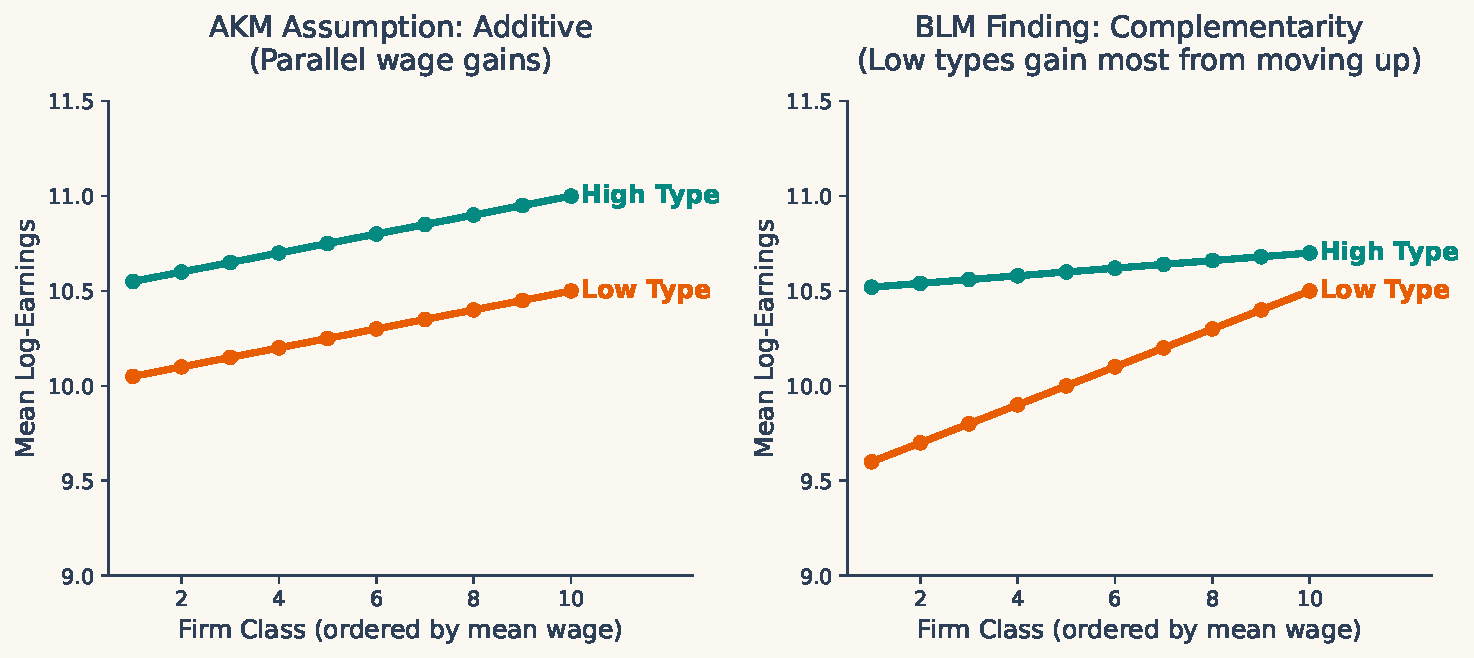
\includegraphics[width=0.95\textwidth]{figures/figure_2.pdf}
    \end{center}
\end{frame}

\transitionslide{By reducing firm heterogeneity to classes, we can tractably identify complex sorting and dynamic wage effects without the incidental parameter bias of AKM.}{}

\appendix
\transitionslide{Appendix}{Mathematical Deep Dive}

\begin{frame}
    \frametitle{Step 1: Grouping firms by minimizing distribution distances}
    
    The $k$-means algorithm partitions $J$ firms into $K$ discrete classes by minimizing:
    
    \[ \min_{k(j), H_k} \sum_{j=1}^J \underbrace{n_j}_{\substack{\text{Workers in} \\ \text{firm } j}} \int \left( \underbrace{\widehat{F}_j(y)}_{\substack{\text{Empirical CDF of} \\ \text{log-wages in } j}} - \underbrace{H_{k(j)}(y)}_{\substack{\text{Latent class } k \\ \text{representative CDF}}} \right)^2 \underbrace{d\mu(y)}_{\substack{\text{Weighting} \\ \text{measure}}} \]
    
    \vspace{0.5cm}
    \begin{itemize}
        \item This identifies firms with similar "wage signatures," regardless of the absolute level of wages.
        \item It reduces the dimensionality from thousands of firms to a handful of classes (e.g., $K=10$).
    \end{itemize}
\end{frame}

\begin{frame}
    \frametitle{The static model allows for type-specific firm premiums}
    
    For a worker $i$ of unobserved type $\alpha_i$ in firm class $k$ at time $t$:
    
    \[ Y_{it} = \underbrace{a_t(k_{it})}_{\substack{\text{Firm class } \\ \text{base premium}}} + \underbrace{b_t(k_{it})}_{\substack{\text{Complementarity} \\ \text{parameter}}} \cdot \underbrace{\alpha_i}_{\substack{\text{Worker} \\ \text{ability type}}} + \underbrace{X_{it}'c_t}_{\substack{\text{Time-varying} \\ \text{observables}}} + \underbrace{\varepsilon_{it}}_{\substack{\text{Idiosyncratic} \\ \text{wage shock}}} \]
    
    \vspace{0.5cm}
    \begin{itemize}
        \item \textbf{AKM nested:} If $b_t(k) = 1$, we have additive separability.
        \item \textbf{Sorting:} Captured by the correlation $Corr(\alpha_i, k_{it})$.
        \item \textbf{Complementarities:} Captured by variation in $b_t(k)$ across classes.
    \end{itemize}
\end{frame}

\begin{frame}
    \frametitle{The dynamic model formalizes endogenous mobility}
    
    The probability of a job move $M_{it}$ depends on the current state:
    
    \[ \underbrace{\Pr(M_{it} = 1 \mid Y_{it}, \alpha_i, k_{it})}_{\text{Mobility Probability}} = \underbrace{\Lambda}_{\text{Logit}} \left( \underbrace{\phi(Y_{it}, \alpha_i, k_{it})}_{\text{Propensity to move}} \right) \]
    
    \vspace{0.3cm}
    And the transition to the next firm class $k_{i,t+1}$:
    
    \[ \underbrace{\Pr(k_{i,t+1} = k' \mid M_{it}=1, Y_{it}, \alpha_i, k_{it})}_{\text{Sorting Transition}} \]
    
    \vspace{0.3cm}
    \textbf{Crucially:} $M_{it}$ depends on $Y_{it}$. If you get a "bad" wage shock ($\varepsilon_{it}$), you are more likely to leave. This violates AKM's strict exogeneity.
\end{frame}

\begin{frame}
    \frametitle{The integrated likelihood for the dynamic model}
    
    We estimate parameters $\theta$ by maximizing the log-likelihood of the observed data:
    
    \[ \log \mathcal{L}(\theta) = \sum_{i=1}^N \log \sum_{\alpha=1}^L \underbrace{\pi(\alpha \mid k_{i1})}_{\substack{\text{Initial sorting:} \\ \text{Type dist. in } k_1}} \prod_{t=1}^{T-1} \underbrace{\mathcal{P}(Y_{it}, M_{it}, k_{i,t+1} \mid Y_{i,t-1}, \alpha, k_{it})}_{\text{Joint density of wages and mobility}} \]
    
    \vspace{0.5cm}
    \begin{itemize}
        \item The inner sum handles the fact that worker type $\alpha$ is \textbf{latent} (Finite Mixture).
        \item The product captures the Markovian transitions over the panel.
        \item Solved via the \textbf{EM algorithm} for computational efficiency.
    \end{itemize}
\end{frame}

\end{document}
